\documentclass[10pt,twoside]{article}

\usepackage[T1]{fontenc}
\usepackage[utf8]{inputenc}
\usepackage{lmodern}
\usepackage[a4paper,margin=2.2cm]{geometry}
\usepackage{graphicx}
\usepackage{booktabs}
\usepackage{amsmath,amssymb}
\usepackage{upgreek}
\usepackage{siunitx}
\usepackage[table]{xcolor}
\usepackage{caption}
\usepackage{microtype}
\usepackage{authblk}
\usepackage[hidelinks]{hyperref}
\usepackage{cleveref}
\emergencystretch=2.5em

\sisetup{detect-all, per-mode=symbol, group-separator={,}}
\captionsetup{font=small, labelfont=bf, width=0.95\textwidth}
\setlength{\parskip}{0.25em}
\graphicspath{{figures/}}

\title{\bfseries Machine-Learning Descriptor Analysis and Bayesian Data
Augmentation for MXene Supercapacitor Capacitance Prediction:\\
Implications for Physics-Guided Modelling}

\author{}
\date{\today}

\begin{document}
\maketitle
\thispagestyle{empty}

\begin{abstract}
\noindent
Literature-derived datasets are an appealing route to data-driven design of MXene
supercapacitor electrodes, but they are small and heterogeneous. We compile 118 usable
gravimetric-capacitance observations for Ti\textsubscript{3}C\textsubscript{2}T\textsubscript{x}
in H\textsubscript{2}SO\textsubscript{4} from 40 publications, standardise thirteen
structural and processing descriptors with unit-aware parsing, and evaluate prediction under
strict publication-grouped cross-validation with a full target-leakage audit. Cross-paper
transferability is weak
($R^2 = 0.03 \pm 0.12$, MAE
$= 82$\,F\,g\textsuperscript{-1}). A variance decomposition localises
the cause: 64\% of the variance in capacitance and a mean of
87\% of the variance in the descriptors lies \emph{between}
publications, and several descriptors are constant within each publication
(ICC$(1)\approx1$). We then test whether Bayesian-network augmentation
(\textsc{DataSynthesizer}, correlated-attribute mode) relieves the small-sample constraint,
fitting the generator inside each training fold only and sweeping four augmentation ratios,
three network degrees and three generator seeds. It does not: the best condition improves MAE
by 6.0\,F\,g\textsuperscript{-1}, less than the
12.3\,F\,g\textsuperscript{-1} obtained by re-drawing the synthetic set alone, with
a non-monotonic response in the amount of synthetic data. The generator itself was faithful
--- no marginal rejected by a Kolmogorov--Smirnov test, Jensen--Shannon distance
0.08 on categorical frequencies, dependency structure
reproduced to $\approx0.06$, and no memorisation of real rows
--- so the null result reflects the nature of the bottleneck rather than a generator failure:
resampling a learned joint distribution cannot supply information about experimental domains
the source papers never visited. SHAP attribution is nevertheless highly stable under this
resampling (Spearman $\rho = 0.90$, top-5 overlap
5/5), which licenses using the real-only ranking for descriptor
prioritisation. Finally we assess what physics the corpus can enforce. A classical
PDE-based physics-informed neural network is not justified --- potential window, discharge
time, current and any time axis are entirely absent --- but two algebraic capacitance closure
identities hold to a median relative error below 1\%, allowing areal and volumetric
capacitance to serve as auxiliary supervised outputs under a hard consistency constraint. We
therefore recommend a hybrid physics-constrained multi-task regression, and identify the
potential window and discharge time as the highest-value missing measurements.
\end{abstract}

\vspace{4pt}
\noindent\textbf{Keywords:} MXene; supercapacitor; gravimetric capacitance; SHAP; Bayesian
network; synthetic data augmentation; domain shift; physics-guided machine learning.


\section{Introduction}\label{sec:intro}

Two-dimensional Ti\textsubscript{3}C\textsubscript{2}T\textsubscript{x} MXene is among the most
studied electrode materials for aqueous supercapacitors~\cite{naguib2011,ghidiu2014}, and a
large body of work reports
gravimetric capacitance in H\textsubscript{2}SO\textsubscript{4} electrolyte. The
accumulated literature is an attractive target for data-driven analysis: if the reported
capacitances could be related to the structural and processing descriptors that accompany
them, the resulting model would both rank the descriptors worth optimising and supply a
data-driven prior for a subsequent physics-informed model.

That programme faces three obstacles that this study addresses directly. First, a corpus
assembled from independent publications is not an experimental design. Cell geometry,
reference electrode, mass-normalisation convention, potential window and reporting rate
differ from paper to paper, and several descriptors are reported at most once per
publication, so the unit of independent information is the paper rather than the row.
Second, such corpora are small: after discarding every entry whose capacitance is reported
only as a range or an inequality, 118 usable observations remain, drawn from 40
publications. Third, the descriptors of greatest physical interest --- interlayer spacing,
surface area, mass loading --- are exactly those most often omitted.

Synthetic data augmentation is a natural response to the second obstacle. A recent study of
flow-capacitive deionisation expanded 32 experimental observations to 200 using the
correlated-attribute (Bayesian-network) mode of \textsc{DataSynthesizer} and reported
improved model performance~\cite{fcdi_augmentation}. Whether that strategy transfers to a
corpus whose limiting factor is heterogeneity rather than row count is an open and
practically important question, and it is the question this work tests.

The contributions are as follows. (i) A leakage-controlled, paper-grouped evaluation of
gravimetric capacitance prediction on the compiled corpus. (ii) A pre-registered test of
Bayesian-network augmentation at four ratios, three network degrees and three independent
generator seeds, in which the generator is fitted inside each training fold only.
(iii) A fidelity audit establishing that the generator reproduces the training distribution
it was shown, so that the augmentation result can be interpreted rather than dismissed as a
generator failure. (iv) A variance decomposition that locates the bottleneck in
between-study heterogeneity. (v) A SHAP descriptor analysis~\cite{shap2017,treeshap2020} whose ranking is shown to be
stable under Bayesian resampling, together with an explicit assessment --- rejecting a
classical PINN~\cite{pinn2019} and specifying the physics-constrained alternative the data
do support.

\section{Dataset and preprocessing}\label{sec:data}

\subsection{Corpus}
The corpus (\texttt{h2so4\_corpus\_final.csv}) contains 192 extracted electrode
records with 83 fields, obtained by structured extraction from published articles reporting
Ti\textsubscript{3}C\textsubscript{2}T\textsubscript{x} performance in
H\textsubscript{2}SO\textsubscript{4}. The prediction target is gravimetric capacitance
$C_g$ in F\,g\textsuperscript{-1}. Table~\ref{tab:dataset} summarises the corpus after
cleaning and Fig.~\ref{fig:dataset} shows its structure.

\subsection{Target cleaning}
A record is retained only when its capacitance is a single defensible number. Values
carrying an approximation marker (\texttt{$\sim$325}, \texttt{about 1.1}) or a mean
$\pm$ standard deviation are retained and flagged. Ranges (\texttt{300--350}) and
inequalities (\texttt{over 200}, \texttt{$<$300}) are \emph{never} collapsed to a
midpoint: 4 such rows were discarded, alongside
70 rows reporting no value.
118 rows from 40 publications survive. Two physically extreme values
(7.26 and 1609.5\,F\,g\textsuperscript{-1})
are retained and flagged rather than deleted; a sensitivity analysis excluding them from
scoring is reported in \texttt{02\_real\_only\_outlier\_sensitivity.csv}.

\subsection{Descriptor standardisation}
Thirteen descriptors were standardised by unit-aware parsing functions rather than manual
editing. Conversions are applied only where the source unit is unambiguous
($\mathrm{nm}\rightarrow\text{\AA}$, $\mathrm{mm}\rightarrow\upmu\mathrm{m}$,
$\upmu\mathrm{g\,cm^{-2}}\rightarrow\mathrm{mg\,cm^{-2}}$,
$\mathrm{V\,s^{-1}}\rightarrow\mathrm{mV\,s^{-1}}$). Incompatible bases are left
missing: a current density reported as mA\,cm\textsuperscript{-2} or
A\,cm\textsuperscript{-3} is not convertible to A\,g\textsuperscript{-1} without
information the corpus does not contain, and a mass loading given in mg or wt.\% carries no
area basis. Electrolyte molarity is parsed from the electrolyte field only; the synthesis
field also contains acid concentrations (e.g.\ wet-spinning in 98\,wt.\%
H\textsubscript{2}SO\textsubscript{4}) that are not the test electrolyte. Free-text
morphology, composition and synthesis strings are mapped to categorical families.
\texttt{synthesis\_family} collapses to a single level (LiF/HCl MILD etching~\cite{alhabeb2017}) among
the surviving rows and is therefore dropped as uninformative, leaving 12 descriptors.

\subsection{Paper grouping and leakage control}
Each row is assigned a \texttt{paper\_id} (DOI where available, else source filename; the
two are one-to-one in this corpus). Of 83 raw columns, 14 are admissible as predictors.
Excluded are volumetric and areal capacitance --- both algebraic transforms of the target
--- together with extraction-confidence and provenance metadata, free-text extraction
rationales that can quote the target value verbatim, publication identifiers, and the
\texttt{role}/\texttt{is\_primary} annotations, which are assigned with knowledge of
the measured performance. No energy- or power-density columns exist in this corpus, so the
usual $E=\tfrac{1}{2}CV^2$ leakage route is absent.

\begin{figure*}[htbp]\centering
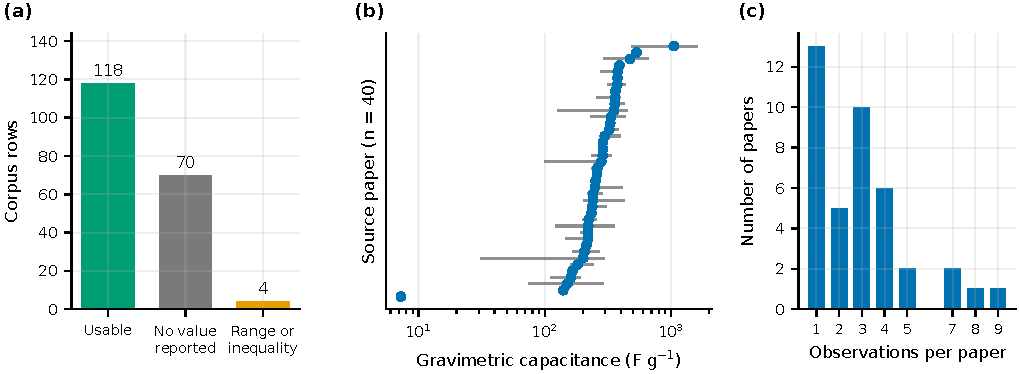
\includegraphics[width=\textwidth]{figures/fig01_dataset_structure.pdf}
\caption{Structure of the compiled corpus. (a) Disposition of the 192 raw records.
(b) Capacitance range of each of the 40 publications (bar: min--max; marker: median),
sorted by median. (c) Distribution of observations per publication. The corpus is a set of
small, tight within-paper clusters spread over a wide global range.}
\label{fig:dataset}\end{figure*}

\begin{table}[htbp]
\centering
\caption{Composition of the literature-derived H\textsubscript{2}SO\textsubscript{4} MXene corpus after target cleaning and descriptor standardisation.}
\label{tab:dataset}
\footnotesize
\begin{tabular}{lr}
\toprule
\textbf{Quantity} & \textbf{Value} \\
\midrule
Rows in the raw corpus & 192 \\
Source publications in the raw corpus & 49 \\
Rows with a usable single-valued $C_g$ & 118 \\
Publications represented after cleaning & 40 \\
Rows dropped: no value reported & 70 \\
Rows dropped: range or inequality literal & 4 \\
Approximate values retained and flagged & 2 \\
Median observations per paper & 3 \\
Maximum observations from one paper & 9 \\
Capacitance range (F\,g\textsuperscript{-1}) & 7.3--1609.5 \\
Capacitance median (F\,g\textsuperscript{-1}) & 266.5 \\
Standardised descriptors retained & 12 \\
Raw columns admissible as predictors & 14 \\
\bottomrule
\end{tabular}
\par\vspace{2pt}\begin{minipage}{\linewidth}\scriptsize Range and inequality literals (e.g.\ \texttt{300--350}, \texttt{over 200}) were discarded rather than converted to midpoints; every discarded row is logged in \texttt{01\_target\_disposition\_log.csv}.\end{minipage}
\end{table}

\section{Machine-learning methodology}\label{sec:methods}

\subsection{Estimator}
Gradient-boosted regression trees (XGBoost~\cite{xgboost2016}) are used throughout. The estimator handles
missing values natively, which matters here because several descriptors are reported by a
minority of papers, and it is robust on the sample sizes involved. Categorical descriptors
are one-hot encoded with an encoder fitted on the training partition only and
\texttt{handle\_unknown="ignore"}, so a level appearing solely in a held-out paper cannot
influence the encoding.

\subsection{Paper-grouped cross-validation}
Ordinary random splitting is inadmissible here. Multiple rows originate from the same
publication and share its cell, protocol and often its exact descriptor values, so a random
split would place near-duplicates on both sides of the partition and report an optimistic
score. All evaluation therefore uses \texttt{GroupKFold} on \texttt{paper\_id} with five
folds: rows from one publication are never split across training and test.

\subsection{Hyper-parameter selection}
Hyper-parameters are chosen by randomised search inside an \emph{inner} paper-grouped
split of the training partition of each outer fold, implemented with
scikit-learn~\cite{sklearn2011}. The outer test papers never influence
model selection, encoding, or any preprocessing statistic. A fixed seed of 42 is used for
NumPy, Python \texttt{random}, XGBoost, the cross-validation splitters and the synthetic
generator.

\subsection{Two models with different purposes}
This is the central methodological distinction of the study and it is maintained throughout.

\begin{itemize}
\item The \textbf{paper-grouped cross-validation} above estimates \emph{predictive
transferability} to publications the model has not seen. It is the only number quoted as a
performance estimate.
\item A \textbf{final real-only interpretation model} is fitted to all 118 usable
observations and is used \emph{solely} to characterise multivariate descriptor
associations within the compiled corpus. Its in-sample fit
($R^2 = 0.624$) is reported here only for
completeness and is not a generalisation estimate.
\end{itemize}

Conflating the two would be the most consequential error available in this analysis, so the
two models are named, stored and reported separately
(\texttt{results\_final/models/model\_card.md}).

\subsection{Metrics}
$R^2$, MAE and RMSE are reported per fold and aggregated as mean, SD and median. Because
$R^2$ is normalised by the variance of each fold's own held-out targets, folds whose papers
happen to agree with one another are scored against a very small denominator; pooled metrics
computed over all held-out predictions jointly are therefore also reported.

\section{Bayesian-network augmentation}\label{sec:bnmethod}

\subsection{Generator}
Synthetic observations are produced with
\textsc{DataSynthesizer}~0.1.13~\cite{datasynthesizer2017} in
\emph{correlated-attribute mode}, which fits a Bayesian network over the attributes by a
greedy mutual-information search~\cite{privbayes2017} and samples from the resulting
factorisation. No substitute
generator (CTGAN, Gaussian copula, SMOTE, KDE) was used at any point. The privacy budget is
set to $\varepsilon = 0$: the inputs are already-published literature values, so
differential-privacy noise would degrade fidelity for no benefit.

\subsection{Attribute treatment}
The network is given 5 descriptors plus the target:
\texttt{h2so4\_M}, \texttt{composition\_family}, \texttt{scan\_rate\_mV\_s}, \texttt{interlayer\_A} and \texttt{layer\_class}.
Electrolyte molarity and scan rate are declared \emph{categorical} despite being numeric:
each occurs at only a handful of discrete experimenter-chosen settings, and a continuous
treatment would let the generator invent molarities and sweep rates that no experiment in
the corpus used. Interlayer spacing and the target remain continuous.

\subsection{Cohort}
Requiring every selected descriptor to be reported in the same publication reduces the
corpus to a complete-case cohort of 47 rows from
18 papers. \textbf{All four training conditions use exactly this
cohort and this feature set}, so the comparison is like-for-like. This cohort model is a
control arm for the augmentation experiment and is not the headline real-only baseline of
Sec.~\ref{sec:grouped}.

\subsection{Anti-leakage protocol}
Within each outer grouped fold the Bayesian network is fitted on the \emph{training papers
only}; synthetic rows are drawn from that network; the physical-validity filter uses
training-fold minima and maxima only; the one-hot encoder and the hyper-parameter search
also see training papers only. Held-out papers are never described, never generated from,
never augmented, and never enter any training set. No synthetic row ever appears in a test
partition.

\subsection{Experimental grid}
Four training conditions are compared: real only, and real plus $1\times$, $3\times$ and
$5.25\times$ synthetic rows, the last reproducing the $200/32 = 6.25$ total-size ratio of the
motivating study. Network degree $k \in \{1,2,3\}$ is swept, with $k=2$ as the
pre-registered default. Each augmented condition is generated three times with independent
generator seeds inside every fold and the fold score is the mean over those draws, so that
re-drawing the synthetic set cannot masquerade as an effect. Generated rows pass a
physical-validity filter (positive capacitance, non-negative descriptors, categorical levels
seen in training, values inside the training-fold range) before use.

\section{Cross-paper prediction results}\label{sec:grouped}

Table~\ref{tab:grouped} and Fig.~\ref{fig:grouped} report the paper-grouped
cross-validation of the real-only model on the full descriptor set. Averaged over folds,
$R^2 = 0.030 \pm 0.119$,
MAE $= 81.5 \pm 32.8$\,F\,g\textsuperscript{-1} and
RMSE $= 129.2 \pm 84.9$\,F\,g\textsuperscript{-1};
pooled over all held-out predictions, $R^2 = 0.081$.
Fold-level $R^2$ ranges from -0.102 to 0.151.

\paragraph{Interpretation of a near-zero and partly negative $R^2$.}
A negative $R^2$ on a fold means the predictions for those held-out papers are worse, under
the coefficient-of-determination criterion, than simply predicting the mean of that fold's
own test targets --- a baseline unavailable in practice, since it requires the answers. It
does not mean the model is uninformative in absolute terms: the mean absolute error of
82\,F\,g\textsuperscript{-1} against a corpus median of
266\,F\,g\textsuperscript{-1} is poor but not vacuous.
What the result does establish is that \emph{cross-paper predictive transferability is
weak}. We report this plainly; it is the central empirical constraint on everything that
follows.

\subsection{Why: cross-study heterogeneity}\label{sec:domainshift}

A one-way variance decomposition by publication (Table~\ref{tab:heterogeneity}) locates the
difficulty. For the target, the between-paper share of total sum-of-squares is
$\eta^2 = 0.64$ with an intraclass correlation of ICC$(1) = 0.47$: most of
the variation in capacitance is variation between publications, not within them.

The descriptors are far more paper-bound still, averaging
$\eta^2 = 0.87$. Several are \emph{paper-level constants}:
electrolyte molarity, gravimetric current density and pore diameter have
ICC$(1) \approx 1$, and layer morphology and synthesis route take a single level within
essentially every publication (mean within-paper purity $1.00$). The median within-paper
range of a numeric descriptor is only
0\% of its global range.

This has a direct consequence for the cross-validation. Holding out a publication removes an
entire descriptor setting rather than a sample from a shared distribution, so the model is
asked to extrapolate to a corner of descriptor space it has never observed. Per fold, the
fraction of held-out capacitances lying inside the training range is
0.92--1.00, and the standardised mean difference between
training and test targets reaches 0.12.

It also has a direct consequence for interpretation, developed in Sec.~\ref{sec:shap}: when
a descriptor is constant within each paper, its apparent importance is statistically
inseparable from the identity of the papers that used that setting.

\begin{figure*}[htbp]\centering
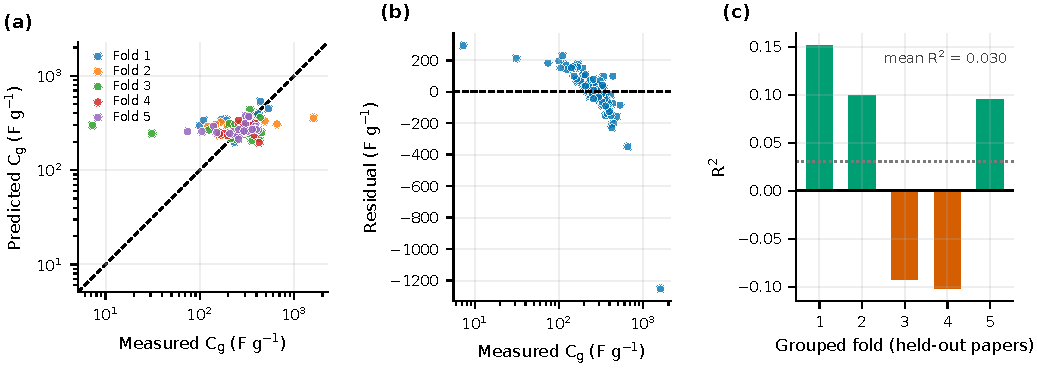
\includegraphics[width=\textwidth]{figures/fig02_grouped_prediction.pdf}
\caption{Paper-grouped cross-validation of the real-only model. (a) Measured versus
predicted capacitance for held-out papers, coloured by fold; the dashed line is parity.
(b) Residuals. (c) Per-fold $R^2$; the dotted line is the mean. Predictions regress towards
the corpus centre, which is the expected behaviour when each fold requires extrapolation to
an unobserved descriptor setting.}
\label{fig:grouped}\end{figure*}

\begin{table}[htbp]
\centering
\caption{Paper-grouped cross-validation of the real-only XGBoost model on the full descriptor set. MAE and RMSE in F\,g\textsuperscript{-1}. Rows from one publication never appear in both the training and test partition.}
\label{tab:grouped}
\footnotesize
\begin{tabular}{lrrrrrr}
\toprule
\textbf{Fold} & \textbf{$n_{\mathrm{train}}$} & \textbf{$n_{\mathrm{test}}$} & \textbf{Papers} & \textbf{$R^2$} & \textbf{MAE} & \textbf{RMSE} \\
\midrule
1 & 94 & 24 & 8 & 0.151 & 61.3 & 90.4 \\
2 & 94 & 24 & 8 & 0.099 & 134.7 & 278.7 \\
3 & 94 & 24 & 8 & -0.092 & 90.3 & 115.7 \\
4 & 95 & 23 & 8 & -0.102 & 52.4 & 73.9 \\
5 & 95 & 23 & 8 & 0.095 & 69.0 & 87.5 \\
\midrule \textbf{Mean} &  &  &  & \textbf{0.030} & \textbf{81.5} & \textbf{129.2} \\
SD &  &  &  & 0.119 & 32.8 & 84.9 \\
Median &  &  &  & 0.095 & 69.0 & 90.4 \\
Pooled &  &  &  & 0.081 & 81.9 & 150.8 \\
\bottomrule
\end{tabular}
\par\vspace{2pt}\begin{minipage}{\linewidth}\scriptsize ``Pooled'' scores every held-out prediction from every fold together, which avoids normalising by a near-zero within-fold target variance while keeping the grouped hold-out intact.\end{minipage}
\end{table}
\begin{table}[htbp]
\centering
\caption{One-way variance decomposition by source publication. $\eta^2$ is the share of total sum-of-squares lying between papers; ICC(1) is the corresponding intraclass correlation corrected for unequal group sizes.}
\label{tab:heterogeneity}
\footnotesize
\begin{tabular}{llrrrr}
\toprule
\textbf{Variable} & \textbf{Role} & \textbf{$n$} & \textbf{Papers} & \textbf{$\eta^2$} & \textbf{ICC(1)} \\
\midrule
current density A g & descriptor & 35 & 16 & 1.000 & 1.000 \\
pore diameter nm & descriptor & 4 & 4 & 1.000 & -- \\
h2so4 M & descriptor & 111 & 38 & 1.000 & 1.000 \\
ssa m2 g & descriptor & 35 & 17 & 0.989 & 0.980 \\
interlayer A & descriptor & 88 & 32 & 0.970 & 0.955 \\
electrode thickness um & descriptor & 54 & 20 & 0.969 & 0.955 \\
flake size um & descriptor & 11 & 6 & 0.727 & 0.493 \\
scan rate mV s & descriptor & 88 & 29 & 0.672 & 0.526 \\
target cap F g & target & 118 & 40 & 0.645 & 0.474 \\
mass loading mg cm2 & descriptor & 55 & 19 & 0.500 & 0.263 \\
\bottomrule
\end{tabular}
\par\vspace{2pt}\begin{minipage}{\linewidth}\scriptsize Values approaching unity mean a variable is essentially constant within a publication and varies only between publications, so holding out a whole paper requires the model to extrapolate rather than interpolate.\end{minipage}
\end{table}

\section{Bayesian augmentation results}\label{sec:augres}

Table~\ref{tab:augmentation} and Fig.~\ref{fig:aug} compare the four training conditions
on the identical set of held-out real papers.

Real-only training on the cohort gives MAE
$= 129.6 \pm 68.0$\,F\,g\textsuperscript{-1}. The
nominally best augmented condition (D, $+5.25\times$) reaches
123.6\,F\,g\textsuperscript{-1}, an improvement of
6.0\,F\,g\textsuperscript{-1}
(-4.6\%), improving MAE in
3 of 5 folds. The $+3\times$ condition
is the \emph{worst} of the four.

\subsection{Why this improvement is not robust}
Three observations, all visible in Fig.~\ref{fig:noise}, place the apparent gain inside the
configuration noise.

\begin{enumerate}
\item \textbf{Re-drawing the synthetic set moves the score by more than the effect.}
Holding fold, ratio and network degree fixed and changing only the generator seed shifts
fold MAE by 12.3\,F\,g\textsuperscript{-1} on average --- larger than the
6.0\,F\,g\textsuperscript{-1} attributed to the best ratio.
\item \textbf{Changing the network degree moves it as much as changing the ratio.} At fixed
ratio, varying $k \in \{1,2,3\}$ changes MAE by up to
17.8\,F\,g\textsuperscript{-1}, while the entire spread across the four
augmentation ratios is 15.1\,F\,g\textsuperscript{-1}. Two nuisance
parameters and the treatment produce effects of the same magnitude.
\item \textbf{The response is not monotone in the amount of synthetic data.} The ordering
is $+5.25\times$, real-only, $+1\times$, $+3\times$. A genuine regularisation benefit would
not place the middle ratio last.
\end{enumerate}

Paired Wilcoxon signed-rank tests across the five folds were computed
(\texttt{06\_statistical\_comparison.csv}), but with five paired folds the smallest
attainable two-sided $p$-value is $2^{-4} = 0.0625$, so no comparison here can reach
$p<0.05$ by construction. The $p$-values are reported for completeness only; the effect
direction, its consistency across folds and its size relative to the noise floor are the
meaningful quantities, and none supports the augmentation.

\paragraph{Conclusion.} Bayesian-network augmentation did not produce robust evidence of
improved prediction on unseen real papers at any ratio tested. This is reported as found: no
configuration search was run to make the synthetic data appear beneficial, and the largest
augmentation ratio was not preferentially reported.

\begin{figure*}[htbp]\centering
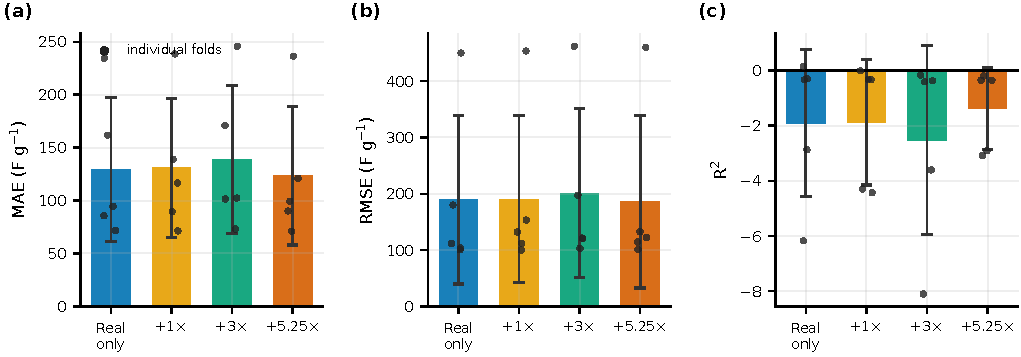
\includegraphics[width=\textwidth]{figures/fig03_augmentation_comparison.pdf}
\caption{Real-only versus augmented training on unseen real papers ($k=2$; bars are means
over five grouped folds, error bars the fold-to-fold SD, points the individual folds).
(a) MAE, (b) RMSE, (c) $R^2$. The conditions are indistinguishable relative to the
fold-to-fold spread.}
\label{fig:aug}\end{figure*}

\begin{figure*}[htbp]\centering
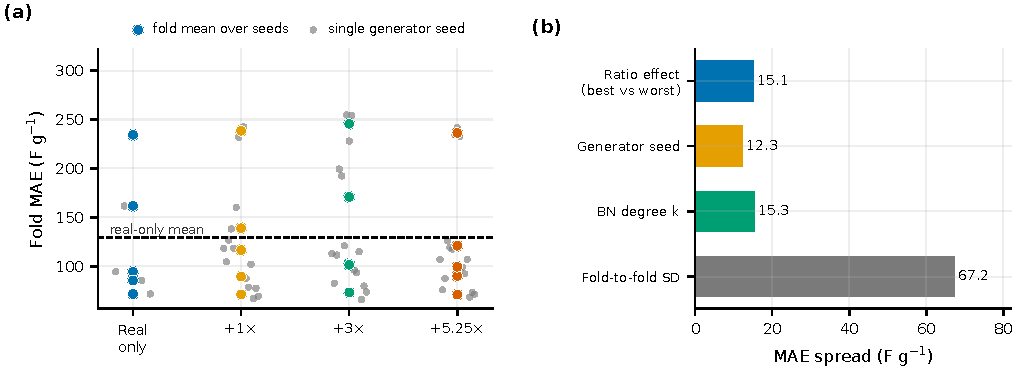
\includegraphics[width=\textwidth]{figures/fig05_generator_uncertainty.pdf}
\caption{The apparent augmentation effect against the noise it must be judged against.
(a) Fold MAE for every generator seed (grey) and the fold mean over seeds (coloured); the
dashed line is real-only training. (b) The best-versus-worst ratio effect compared with the
spread produced by re-drawing the synthetic set, by changing the Bayesian-network degree, and
by fold-to-fold variation. The treatment effect is indistinguishable in magnitude from the two
nuisance sources and is an order of magnitude below the fold-to-fold spread.}
\label{fig:noise}\end{figure*}

\begin{table}[htbp]
\centering
\caption{Real-only versus Bayesian-augmented training, evaluated on the identical set of held-out real papers in every condition ($k=2$, five grouped folds, three independent generator seeds averaged per fold). Errors in F\,g\textsuperscript{-1}; $\pm$ denotes the fold-to-fold SD.}
\label{tab:augmentation}
\footnotesize
\begin{tabular}{lrrrrrr}
\toprule
\textbf{Training set} & \textbf{$n_{\mathrm{syn}}$} & \textbf{$R^2$} & \textbf{MAE} & \textbf{RMSE} & \textbf{Pooled MAE} & \textbf{Seed SD} \\
\midrule
Real only & 0 & -1.91 $\pm$ 2.67 & 129.6 $\pm$ 68.0 & 189.1 $\pm$ 149.3 & 129.5 & -- \\
Real $+\,1\times$ & 38 & -1.88 $\pm$ 2.27 & 130.9 $\pm$ 65.4 & 190.2 $\pm$ 148.6 & 130.8 & 11.1 \\
Real $+\,3\times$ & 113 & -2.53 $\pm$ 3.43 & 138.7 $\pm$ 69.8 & 200.8 $\pm$ 150.3 & 138.6 & 18.9 \\
Real $+\,5.25\times$ & 198 & -1.38 $\pm$ 1.48 & 123.6 $\pm$ 65.5 & 186.1 $\pm$ 153.5 & 122.8 & 6.9 \\
\bottomrule
\end{tabular}
\par\vspace{2pt}\begin{minipage}{\linewidth}\scriptsize ``Seed SD'' is the within-fold MAE standard deviation across the three generator seeds, i.e.\ the score movement produced by re-drawing the synthetic set alone. It is of the same magnitude as the entire spread between augmentation ratios, and for the $+3\times$ condition it exceeds it.\end{minipage}
\end{table}

\section{Synthetic-data fidelity}\label{sec:fidelity}

A null augmentation result is only informative if the generator itself worked. Every metric
below compares synthetic rows against the real training rows \emph{of the same fold}, never
the test papers (Table~\ref{tab:fidelity}, Fig.~\ref{fig:fid}).

\paragraph{Marginals.} The mean Kolmogorov--Smirnov statistic is
0.154 and \textbf{no} continuous variable was rejected at
$p<0.05$ in any fold, ratio or seed.

\paragraph{Categorical frequencies.} The mean Jensen--Shannon distance is
0.079, indicating close agreement of level frequencies.

\paragraph{Dependency structure.} The Pearson correlation matrix differs by
0.047 in mean absolute value and the normalised
mutual-information matrix, which also covers the categorical descriptors, by
0.055.

\paragraph{Descriptor--target relationships.} This is the fidelity criterion that matters
most for downstream utility, since a generator can match every marginal and still destroy the
relationship a regressor must learn. Measured as Spearman correlation with the target for
continuous descriptors and $\eta^2$ for categorical ones, the mean absolute change is
0.065.

\paragraph{Memorisation.} Across all folds, ratios and seeds,
0 synthetic rows were exact copies of a real
training row and 0 were duplicated within a
synthetic set. The median synthetic-to-real nearest-neighbour distance is
0.33 times the median
real-to-real distance. A ratio below unity is expected rather than alarming here, since
37--200 synthetic points are drawn
over the same manifold as 37 real ones and
nearest-neighbour distances contract with density alone; the sharper diagnostic is that only
3.5 of
116 synthetic rows on average fall closer to a real record than
the fifth percentile of real-to-real spacing.

\paragraph{Central interpretation.} The generator reproduced the joint distribution it was
shown, and did so without copying. \textbf{Distributional fidelity to the training fold does
not imply improved generalisation to a held-out publication.} A Bayesian network resamples
the dependencies present in its training data; it cannot supply information about
experimental domains the training papers never visited. Since Sec.~\ref{sec:domainshift}
establishes that the held-out papers are precisely such unvisited domains, the null result of
Sec.~\ref{sec:augres} is the expected outcome rather than an anomaly, and it is not
attributable to a defective generator.

\begin{figure*}[htbp]\centering
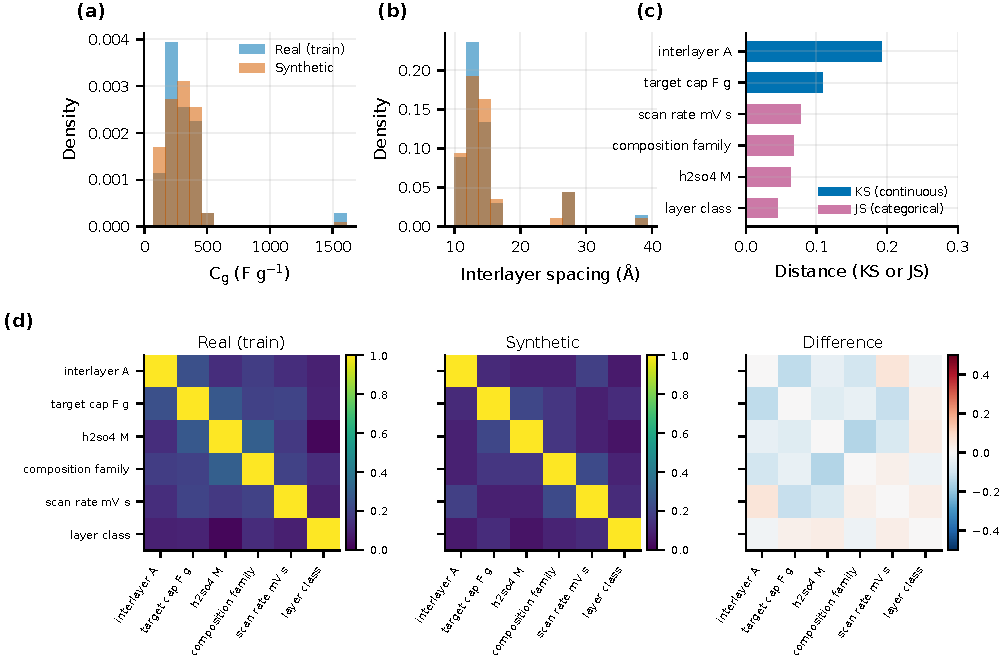
\includegraphics[width=\textwidth]{figures/fig04_synthetic_fidelity.pdf}
\caption{Fidelity of the Bayesian-resampled observations against the real training rows of
the same fold. (a) Target marginal, (b) interlayer-spacing marginal, (c) per-variable
Kolmogorov--Smirnov (continuous) and Jensen--Shannon (categorical) distances, (d) normalised
mutual-information matrices for real and synthetic data and their difference.}
\label{fig:fid}\end{figure*}

\begin{table}[htbp]
\centering
\caption{Fidelity of the Bayesian-network synthetic observations, computed against the real training rows of the same fold ($k=2$; mean, min and max over folds, augmentation ratios and generator seeds).}
\label{tab:fidelity}
\footnotesize
\begin{tabular}{lrrr}
\toprule
\textbf{Fidelity metric} & \textbf{Mean} & \textbf{Min} & \textbf{Max} \\
\midrule
Mean KS statistic (continuous) & 0.154 & 0.095 & 0.198 \\
Continuous variables with KS $p<0.05$ & 0.0 & 0.0 & 0.0 \\
Mean Jensen--Shannon distance (categorical) & 0.079 & 0.028 & 0.170 \\
Pearson correlation matrix, mean $|\Delta|$ & 0.047 & 0.002 & 0.346 \\
Spearman correlation matrix, mean $|\Delta|$ & 0.095 & 0.001 & 0.292 \\
Mutual-information matrix, mean $|\Delta|$ & 0.055 & 0.025 & 0.093 \\
Descriptor--target association, mean $|\Delta|$ & 0.065 & 0.010 & 0.263 \\
Exact duplicates of a real training row & 0.0 & 0.0 & 0.0 \\
Duplicates within a synthetic set & 0.0 & 0.0 & 0.0 \\
Synthetic$\rightarrow$real NN distance (median) & 0.0065 & 0.0046 & 0.0086 \\
Real$\rightarrow$real NN distance (median) & 0.0195 & 0.0130 & 0.0351 \\
\bottomrule
\end{tabular}
\par\vspace{2pt}\begin{minipage}{\linewidth}\scriptsize Nearest-neighbour distances use a range-normalised mixed-type (Gower) metric. No synthetic row reproduced a real training row exactly.\end{minipage}
\end{table}

\section{Real-only SHAP descriptor analysis}\label{sec:shap}

SHAP values~\cite{shap2017} are computed with \texttt{TreeExplainer}~\cite{treeshap2020}
on the final real-only interpretation model fitted to all 118 usable observations (Sec.~\ref{sec:methods}). One-hot columns are
reported individually and aggregated back to the parent descriptor by summing $|$SHAP$|$
within each row before averaging. This is an \emph{association} analysis within the compiled
corpus, not a causal or predictive claim.

\subsection{Descriptor ranking}
Table~\ref{tab:shap} and Fig.~\ref{fig:shapimp} give the ranking. The five leading
descriptors, with their share of total attribution, are: composition family (22\%); H\textsubscript{2}SO\textsubscript{4} concentration (M) (20\%); scan rate (mV\,s\textsuperscript{-1}) (16\%); interlayer spacing (\AA) (10\%); layer morphology (9\%). The ranking agrees closely with
the independent fold-wise held-out SHAP computed during cross-validation: the top five
descriptors each entered the fold-level top five in
80--100\%
of folds.

\subsection{Direction of the associations}
Fig.~\ref{fig:shapbee} and Fig.~\ref{fig:shapdep} show directionality. Higher
H\textsubscript{2}SO\textsubscript{4} concentration is associated with higher predicted
capacitance ($\rho = +0.72$ between the
descriptor value and its own SHAP value), consistent with greater proton availability for
Ti--O pseudocapacitance~\cite{lukatskaya2017}. Higher scan rate is associated with lower predicted capacitance
($\rho = -0.93$), consistent with
rate-limited ion access to the interlayer galleries.

\paragraph{A trend that contradicts the naive expectation.} Interlayer spacing is associated
with \emph{lower} predicted capacitance
($\rho = -0.75$), the opposite of the expectation that a wider gallery eases ion
access. We do not report this as a physical finding. Two confounds are more plausible: the
largest reported $d$-spacings in this corpus belong predominantly to pillared and composite
architectures whose \emph{gravimetric} capacitance is diluted by the mass of the
intercalant, and $d$-spacing is conventionally measured on a dry film rather than in the
hydrated, polarised state in which charge is actually stored. This is a concrete illustration
of why a monotonicity prior must not be read off a SHAP plot.

\paragraph{The confounding caveat, stated quantitatively.} Sec.~\ref{sec:domainshift}
showed that several descriptors are paper-level constants. Electrolyte molarity, the
second-ranked descriptor, has ICC$(1) = 1.00$: it does not vary at
all within a publication. Its SHAP attribution therefore cannot be statistically separated
from the identity of the publications that used each molarity, and the same applies to
interlayer spacing (\AA), current density (A\,g\textsuperscript{-1}), electrode thickness ($\upmu$m) and specific surface area (m\textsuperscript{2}\,g\textsuperscript{-1}). The ranking
should be read as ``descriptors along which the corpus is organised and which the model
exploits'', not as ``levers that would change capacitance if turned''. Distinguishing the two
requires controlled experiments that vary one descriptor within a single laboratory
protocol --- which is precisely what the corpus lacks.

\begin{figure}[htbp]\centering
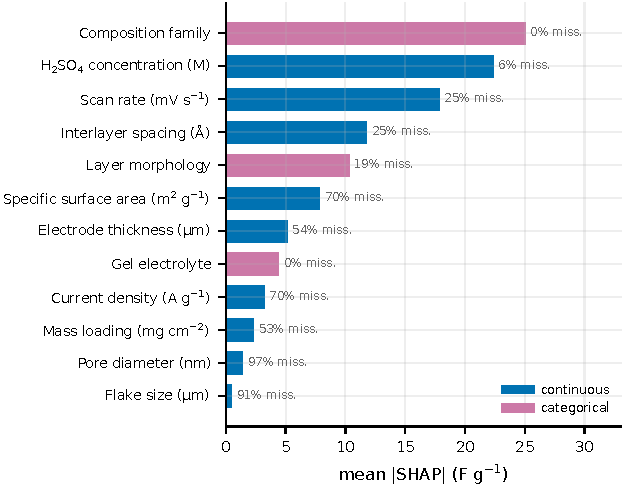
\includegraphics[width=\columnwidth]{figures/fig06_real_shap_importance.pdf}
\caption{Descriptor-level SHAP importance of the final real-only interpretation model.
Bars are the mean absolute SHAP value; annotations give the fraction of observations for
which the descriptor is not reported.}
\label{fig:shapimp}\end{figure}

\begin{figure}[htbp]\centering
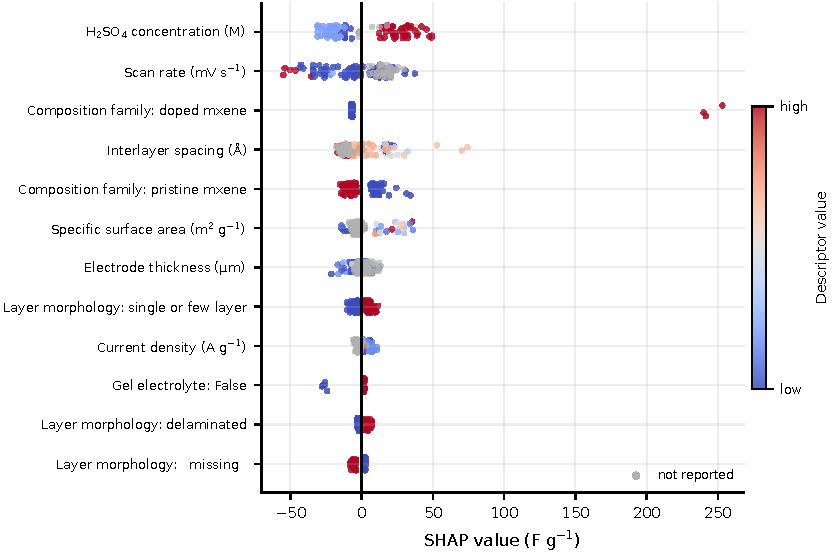
\includegraphics[width=\columnwidth]{figures/fig07_real_shap_beeswarm.pdf}
\caption{SHAP value distribution per encoded feature, coloured by descriptor value. Grey
points are observations for which the descriptor is not reported.}
\label{fig:shapbee}\end{figure}

\begin{figure*}[htbp]\centering
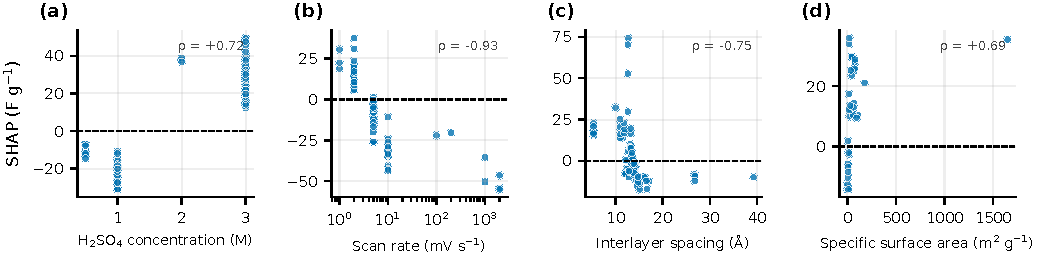
\includegraphics[width=\textwidth]{figures/fig07b_real_shap_dependence.pdf}
\caption{SHAP dependence for the leading continuous descriptors. $\rho$ is the Spearman
correlation between the descriptor value and its own SHAP contribution. The negative trend in
interlayer spacing runs against the naive physical expectation and is discussed in the text.}
\label{fig:shapdep}\end{figure*}

\begin{table}[htbp]
\centering
\caption{Descriptor-level SHAP attribution of the final real-only interpretation model fitted to all usable real observations. $\overline{|\mathrm{SHAP}|}$ in F\,g\textsuperscript{-1}; share, missingness and top-5 frequency in per cent.}
\label{tab:shap}
\footnotesize
\begin{tabular}{rlrrrrrrr}
\toprule
\textbf{Rank} & \textbf{Descriptor} & \textbf{$\overline{|\mathrm{SHAP}|}$} & \textbf{Share} & \textbf{Miss.} & \textbf{Fold rank} & \textbf{Rank SD} & \textbf{Top-5} & \textbf{$\rho$} \\
\midrule
1 & Composition family & 25.05 & 22.3 & 0 & 2.4 & 0.89 & 100 & -- \\
2 & H\textsubscript{2}SO\textsubscript{4} conc.\ (M) & 22.37 & 19.9 & 6 & 1.4 & 0.89 & 100 & 0.72 \\
3 & Scan rate (mV\,s$^{-1}$) & 17.87 & 15.9 & 25 & 2.8 & 1.10 & 100 & -0.93 \\
4 & Interlayer spacing (\AA) & 11.78 & 10.5 & 25 & 4.0 & 1.58 & 80 & -0.75 \\
5 & Layer morphology & 10.31 & 9.2 & 19 & 4.8 & 0.45 & 100 & -- \\
6 & Specific surface area (m$^2$\,g$^{-1}$) & 7.85 & 7.0 & 70 & 6.4 & 1.52 & 20 & 0.69 \\
7 & Electrode thickness ($\upmu$m) & 5.14 & 4.6 & 54 & 7.0 & 1.00 & 0 & -0.23 \\
8 & Gel electrolyte & 4.43 & 3.9 & 0 & 10.0 & 2.00 & 0 & -- \\
9 & Current density (A\,g$^{-1}$) & 3.23 & 2.9 & 70 & 7.8 & 1.48 & 0 & 0.04 \\
10 & Mass loading (mg\,cm$^{-2}$) & 2.33 & 2.1 & 53 & 9.6 & 0.89 & 0 & -0.07 \\
\bottomrule
\end{tabular}
\par\vspace{2pt}\begin{minipage}{\linewidth}\scriptsize ``Fold rank'' and ``Rank SD'' come from the independent held-out SHAP computation of the paper-grouped cross-validation; ``Top-5'' is the fraction of folds in which the descriptor entered the five most important. $\rho$ is the Spearman correlation between a descriptor's value and its own SHAP value (direction of the association, not a causal claim); it is defined for continuous descriptors only.\end{minipage}
\end{table}

\section{SHAP robustness under augmentation}\label{sec:stability}

Although augmentation did not improve prediction, it provides a useful perturbation test: if
the descriptor hierarchy survives having the training set resampled from a learned Bayesian
network, it is not an artefact of the particular rows sampled.

Comparing the cohort real-only model with the best-performing augmented model on the identical
cohort and feature set (Fig.~\ref{fig:stab}):

\begin{itemize}
\item Spearman rank correlation of descriptor rankings:
$\rho = 0.90$ ($p = 0.037$).
\item Top-3 overlap 3/3; top-5 overlap 5/5.
\item Mean absolute rank displacement 0.4 positions
(maximum 1).
\item Mean absolute change in each descriptor's share of total attribution:
0.018.
\end{itemize}

The descriptor hierarchy is therefore stable. This matters for the argument of this paper: the
same experiment that fails to improve prediction succeeds in demonstrating that the
\emph{relative} descriptor ordering is robust to resampling of the training distribution.
Had augmentation improved $R^2$ while substantially reordering the descriptors, that would
have indicated synthetic-distribution distortion and the ranking would not be usable; the
observed combination --- no predictive gain, high attribution stability --- is the one that
licenses using the real-only SHAP ranking for descriptor selection.

\begin{figure*}[htbp]\centering
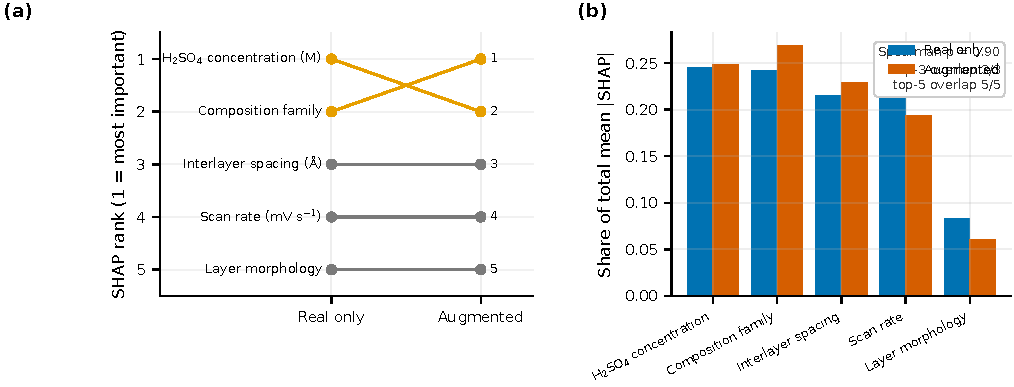
\includegraphics[width=\textwidth]{figures/fig08_shap_stability.pdf}
\caption{Descriptor attribution before and after Bayesian augmentation. (a) Rank slope chart;
grey lines indicate unchanged rank. (b) Share of total mean $|$SHAP$|$ per descriptor.}
\label{fig:stab}\end{figure*}

\section{Implications for physics-informed modelling}\label{sec:pinn}

\subsection{Which quantities the corpus actually contains}
Table~\ref{tab:physavail} audits the corpus against the quantities required by the standard
capacitance relations. The galvanostatic definition
\begin{equation}
C_g = \frac{I\,\Delta t}{m\,\Delta V}
\qquad\text{equivalently}\qquad
C_g = \frac{j\,\Delta t}{\Delta V},
\label{eq:gcd}
\end{equation}
and the cyclic-voltammetry relation
\begin{equation}
C_g = \frac{\int I(V)\,\mathrm{d}V}{m\,\nu\,\Delta V},
\label{eq:cv}
\end{equation}
both require a potential window $\Delta V$. That quantity, together with the discharge time
$\Delta t$, the absolute current $I$, the absolute electrode mass $m$, the electrode area and
the integrated CV current, is \textbf{entirely absent} from the corpus
(\texttt{electrode\_area\_cm2}, \texttt{voltage\_window\_V}, \texttt{current\_A}, \texttt{discharge\_time\_s}, all at
0\% coverage). The corpus does not even record whether a given row is a galvanostatic or a
voltammetric measurement.

\subsection{Assessment of three candidate model classes}
\paragraph{(A) Classical PDE/ODE-based PINN --- not justified.}
A physics-informed neural network in the usual sense~\cite{pinn2019} minimises the residual of
a differential
equation at collocation points, which requires a state variable defined over a space or time
coordinate together with initial and boundary conditions per observation. Every row in this
corpus is a single scalar summary of a completed experiment: there is no time axis, no
potential axis, no spatial coordinate and no trajectory. Without $\Delta V$ and $\Delta t$
even the \emph{algebraic} relation~\eqref{eq:gcd} cannot be evaluated for a single row,
let alone a differential form. Posing a PDE residual here would mean inventing physics rather
than enforcing it, and we therefore reject this option explicitly.

\paragraph{(B) Physics-guided neural network --- feasible.}
Positivity of capacitance, training-domain bounds and dimensionally meaningful inputs are all
available. Monotonicity constraints, however, should \emph{not} be imposed: the corpus shows
an interlayer-spacing trend opposite to the naive expectation (Sec.~\ref{sec:shap}), and
imposing a monotone prior from SHAP would encode a probable confound as physics.

\paragraph{(C) Hybrid physics-constrained multi-task regression --- recommended.}
Two exact algebraic closure identities relate the target to other measured quantities:
\begin{align}
C_A &= C_g\, m_A, \label{eq:areal}\\
C_V &= C_g\, \rho, \qquad \rho = m_A / t, \label{eq:vol}
\end{align}
where $m_A$ is areal mass loading, $t$ electrode thickness and $\rho$ the electrode density.
We verified both against the values reported in the source publications
(Table~\ref{tab:closure}). Equation~\eqref{eq:areal} reproduces the reported areal
capacitance with a median relative error of 0.38\% and holds within
5\% for 85\% of 39 testable rows;
Eq.~\eqref{eq:vol} has a median error of 0.87\% and holds within
5\% for 76\% of 34 rows.

This yields a structural insight that reframes two of the excluded columns. Areal and
volumetric capacitance cannot be \emph{predictors} --- they are algebraic transforms of the
target and were correctly removed as leakage --- but they can serve as \textbf{auxiliary
supervised outputs}, tied to the primary output by Eqs.~\eqref{eq:areal}
and~\eqref{eq:vol}. Two leakage columns thereby become additional training signal and a
genuine internal-consistency constraint, with no leakage introduced.

\subsection{Descriptor classification}
Table~\ref{tab:pinn} classifies every standardised descriptor.
\textbf{Category A} (physics-grade inputs): interlayer spacing (\AA), scan rate (mV\,s\textsuperscript{-1}), mass loading (mg\,cm\textsuperscript{-2}), electrode thickness ($\upmu$m) and H\textsubscript{2}SO\textsubscript{4} concentration (M). Mass loading and electrode
thickness qualify despite modest standalone SHAP importance because they appear directly in
the verified closure identities, entering the physics term rather than the data term.
\textbf{Category B} (machine-learning covariates only): layer morphology, composition family and gel electrolyte --- informative for
prediction, but categorical buckets with no counterpart in any governing relation, and
therefore excluded from every physics term.
\textbf{Category C} (excluded): current density (A\,g\textsuperscript{-1}), specific surface area (m\textsuperscript{2}\,g\textsuperscript{-1}), flake size ($\upmu$m), pore diameter (nm) and synthesis route, on grounds of
sparsity, absent variation, or non-convertible units, in addition to all target-derived and
metadata columns.

\subsection{Proposed formulation}
The recommended next-stage model (Fig.~\ref{fig:model}) predicts $\hat C_g$ through a
softplus output head, guaranteeing positivity by construction, with auxiliary heads for
$\hat C_A$ and $\hat C_V$. The objective is
\begin{equation}
\mathcal{L} = \lambda_{d}\mathcal{L}_{\mathrm{data}}
+ \lambda_{p}\mathcal{L}_{\mathrm{phys}}
+ \lambda_{b}\mathcal{L}_{\mathrm{bound}}
+ \lambda_{r}\lVert\theta\rVert^{2},
\label{eq:loss}
\end{equation}
with
\begin{align}
\mathcal{L}_{\mathrm{data}} &= \frac{1}{N}\sum_{i}
  \mathrm{Huber}\!\left(\hat C_{g,i}, C_{g,i}\right)
  + \sum_{o \in \{A,V\}} \frac{w_o}{|S_o|}\sum_{i \in S_o}
  \mathrm{Huber}\!\left(\hat C_{o,i}, C_{o,i}\right), \\
\mathcal{L}_{\mathrm{phys}} &= \frac{1}{|S_A|}\sum_{i \in S_A}
  \bigl(\hat C_{A,i} - \hat C_{g,i} m_{A,i}\bigr)^{2}
  + \frac{1}{|S_V|}\sum_{i \in S_V}
  \bigl(\hat C_{V,i} - \hat C_{g,i} m_{A,i}/t_i\bigr)^{2}, \\
\mathcal{L}_{\mathrm{bound}} &= \frac{1}{N}\sum_{i}
  \bigl[\max(0, -\hat C_{g,i})\bigr]^{2}
  + \frac{1}{N}\sum_{i} d_{\mathrm{hull}}(\mathbf{x}_i)^{2},
\end{align}
where $S_A$ and $S_V$ index the rows for which the required quantities are actually reported.
All physics residuals are masked in this way, so no value is imputed in order to satisfy a
constraint. A Huber data term is used rather than squared error because the corpus retains
genuine extreme values that a quadratic loss would allow to dominate. Evaluation remains
paper-grouped, and no synthetic rows are used.

\subsection{What would help most}
Table~\ref{tab:physavail} identifies the binding constraint, and the priority list in
\texttt{data\_gap\_priorities.csv} ranks the remedies. The two
highest-value additions are \emph{potential window} and \emph{discharge time}: at 0\%
coverage they are the only missing terms of Eq.~\eqref{eq:gcd}, and recovering them would
promote the physics term from a definitional unit closure applicable to a minority of rows to
the actual measurement equation applicable to every galvanostatic row. Recording the testing
mode would additionally separate galvanostatic from voltammetric measurements, which are
currently pooled.

\begin{figure*}[htbp]\centering
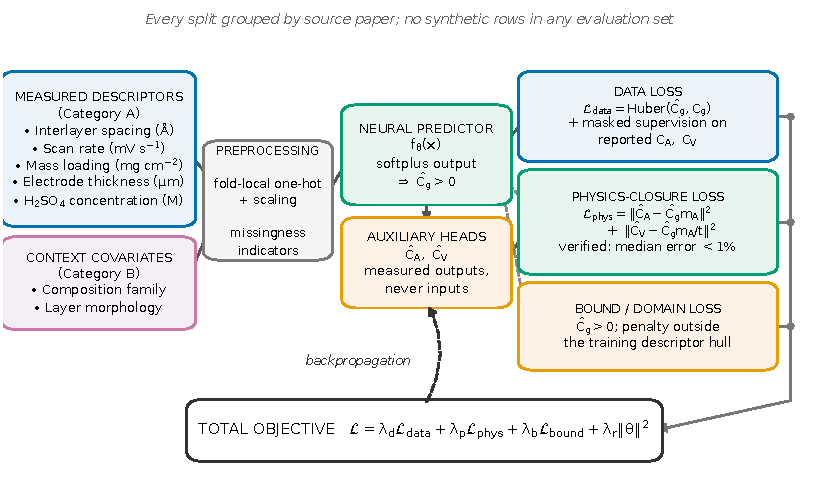
\includegraphics[width=\textwidth]{figures/fig09_proposed_physics_model.pdf}
\caption{Proposed hybrid physics-constrained multi-task architecture. Category~A descriptors
enter the predictor; Category~B covariates enter the data term only. Areal and volumetric
capacitance are auxiliary \emph{outputs}, never inputs, and are tied to the primary output by
the closure identities of Eqs.~\eqref{eq:areal}--\eqref{eq:vol}, which were verified against
the published values.}
\label{fig:model}\end{figure*}

\begin{table}[htbp]
\centering
\caption{Availability of the quantities required by the standard electrochemical capacitance relations, evaluated over the usable real observations.}
\label{tab:physavail}
\footnotesize
\begin{tabular}{llrrl}
\toprule
\textbf{Variable} & \textbf{Symbol} & \textbf{$n$} & \textbf{Coverage (\%)} & \textbf{Usable now} \\
\midrule
h2so4 M & $c0$ & 111 & 94 & yes \\
scan rate mV s & $nu$ & 88 & 75 & yes \\
interlayer A & $d$ & 88 & 75 & yes \\
volumetric capacitance F cm3 & $C\_V$ & 65 & 55 & yes \\
mass loading mg cm2 & $m\_A$ & 55 & 47 & partial - only 47\% of rows \\
electrode thickness um & $t$ & 54 & 46 & partial - only 46\% of rows \\
areal capacitance F cm2 & $C\_A$ & 46 & 39 & partial - only 39\% of rows \\
current density A g & $j$ & 35 & 30 & partial - only 30\% of rows \\
ssa m2 g & $S$ & 35 & 30 & partial - only 30\% of rows \\
electrode area cm2 & $A$ & 0 & 0 & no - variable is not present in the corpus at all \\
voltage window V & $dV$ & 0 & 0 & no - variable is not present in the corpus at all \\
current A & $I$ & 0 & 0 & no - variable is not present in the corpus at all \\
discharge time s & $dt$ & 0 & 0 & no - variable is not present in the corpus at all \\
electrode mass g & $m$ & 0 & 0 & no - variable is not present in the corpus at all \\
testing mode & -- & 0 & 0 & no - variable is not present in the corpus at all \\
cv current integral & $int(I dV)$ & 0 & 0 & no - variable is not present in the corpus at all \\
\bottomrule
\end{tabular}
\par\vspace{2pt}\begin{minipage}{\linewidth}\scriptsize Coverage is the fraction of usable rows for which the quantity can be parsed with an unambiguous unit. The four quantities required by $C_g = I\,\Delta t/(m\,\Delta V)$ that are entirely absent from the corpus are the reason a classical PDE-based PINN cannot presently be posed.\end{minipage}
\end{table}
\begin{table}[htbp]
\centering
\caption{Empirical verification of the algebraic capacitance closure identities against the values reported in the source publications. These identities are the physics that the corpus can actually enforce.}
\label{tab:closure}
\footnotesize
\begin{tabular}{lrrrrrr}
\toprule
\textbf{Closure identity} & \textbf{$n$ rows} & \textbf{Papers} & \textbf{Median err.\ (\%)} & \textbf{$<5\%$} & \textbf{$<20\%$} & \textbf{$>50\%$} \\
\midrule
$C_A = C_g \cdot m_A$ & 39 & 14 & 0.38 & 85 & 90 & 3 \\
$C_V = C_g \cdot m_A /t$ & 34 & 13 & 0.87 & 76 & 85 & 4 \\
\bottomrule
\end{tabular}
\par\vspace{2pt}\begin{minipage}{\linewidth}\scriptsize $m_A$ is areal mass loading and $t$ electrode thickness, so $m_A/t$ is the electrode density. Rows failing by more than 50\% are dominated by publications whose mass-loading convention differs from the one implied by their reported areal capacitance, which is itself evidence of cross-study protocol heterogeneity.\end{minipage}
\end{table}
\begin{table}[htbp]
\centering
\caption{Classification of every standardised descriptor for the next-stage physics-guided model. Category A: physically meaningful, well-covered and stable inputs. Category B: informative machine-learning covariates that are categorical proxies rather than physical parameters. Category C: excluded.}
\label{tab:pinn}
\footnotesize
\begin{tabular}{lrrlll}
\toprule
\textbf{Descriptor} & \textbf{SHAP rank} & \textbf{Miss.\ (\%)} & \textbf{Stability} & \textbf{Category} & \textbf{PINN input?} \\
\midrule
H\textsubscript{2}SO\textsubscript{4} conc.\ (M) & 2 & 6 & stable & A & yes \\
Scan rate (mV\,s$^{-1}$) & 3 & 25 & moderately stable & A & yes \\
Interlayer spacing (\AA) & 4 & 25 & moderately stable & A & yes \\
Electrode thickness ($\upmu$m) & 7 & 54 & stable & A & yes (closure) \\
Mass loading (mg\,cm$^{-2}$) & 10 & 53 & stable & A & yes (closure) \\
Composition family & 1 & 0 & stable & B & not directly \\
Layer morphology & 5 & 19 & stable & B & not directly \\
Gel electrolyte & 8 & 0 & unstable & B & not directly \\
Specific surface area (m$^2$\,g$^{-1}$) & 6 & 70 & moderately stable & C & no \\
Current density (A\,g$^{-1}$) & 9 & 70 & moderately stable & C & no \\
Pore diameter (nm) & 11 & 97 & moderately stable & C & no \\
Flake size ($\upmu$m) & 12 & 91 & moderately stable & C & no \\
Synthesis route & -- & 0 & not assessed & C & no \\
\bottomrule
\end{tabular}
\par\vspace{2pt}\begin{minipage}{\linewidth}\scriptsize Stability combines the cross-fold SHAP rank spread with the rank change observed between the real-only and Bayesian-augmented models. Full reasoning is in \texttt{results\_final/pinn/descriptor\_classification.csv}.\end{minipage}
\end{table}

\section{Discussion}\label{sec:discussion}

\subsection{More rows are not more information}
The central finding of this study is a distinction between sample size and independent
information. The corpus contains 118 rows but only 40 independent experimental contexts,
and 64\% of the variance in capacitance lies between those contexts rather than
within them. Bayesian-network resampling multiplies rows while holding the number of contexts
fixed. Since the generator's joint distribution is estimated from the training papers alone,
every synthetic observation is a recombination of dependencies those papers already exhibit.
When the test partition is a \emph{different} publication --- with its own protocol, its own
mass-normalisation convention and, as Sec.~\ref{sec:domainshift} shows, frequently its own
unique descriptor settings --- no amount of resampling can supply the missing information.
The augmentation null result and the fidelity success are therefore two aspects of the same
fact rather than a contradiction.

This also delimits when the motivating FCDI-style strategy should be expected to work. Where
observations are exchangeable draws from one experimental campaign, resampling the joint
distribution is a reasonable regulariser. Where they are clustered by study and evaluation is
across studies, it addresses the wrong bottleneck.

\subsection{Four purposes that must not be mixed}
The analysis maintains four separate roles, and much of the interpretive risk in this problem
comes from conflating them. \emph{Predictive assessment} uses paper-grouped
cross-validation. \emph{Descriptor interpretation} uses the final real-only model fitted to
all observations. \emph{Robustness testing} uses Bayesian augmentation and SHAP-ranking
stability. \emph{Physics-model design} uses descriptors supported by all three. In
particular, the in-sample fit of the interpretation model is never quoted as performance, and
the stability of the SHAP ranking is never taken as evidence that the model predicts well ---
it does not.

\subsection{Attribution, association and causation}
SHAP quantifies how a fitted model distributes credit among its inputs. Within this corpus
that attribution is stable and reproducible, which makes it a defensible basis for
prioritising descriptors. It is not evidence of causation, and Sec.~\ref{sec:shap} gives a
quantitative reason for caution specific to this dataset: several highly ranked descriptors
are paper-level constants (ICC$(1) \approx 1$), so their attribution is statistically
entangled with publication identity. The interlayer-spacing trend, which runs opposite to the
naive physical expectation, is the clearest symptom. The appropriate conclusion is that these
descriptors organise the corpus and the model uses them, not that changing them would change
measured capacitance.

\subsection{What the physics analysis changes}
Rejecting a classical PINN is a substantive result rather than a negative one. It redirects
effort from constructing a differential residual the data cannot support towards two things
the data do support: enforcing the verified closure identities of
Eqs.~\eqref{eq:areal}--\eqref{eq:vol} as internal-consistency constraints, and extending
the extraction schema to recover the potential window and discharge time. The second is the
higher-value action. It converts the physics term from a unit-consistency relation applicable
to a minority of rows into the measurement equation itself, and it simultaneously addresses
the heterogeneity diagnosis, because knowing $\Delta V$ and the testing mode removes two known
and currently unmodelled sources of between-study scatter.

\subsection{Implications for reporting practice}
The rows discarded during cleaning are themselves a finding. Capacitance reported only as a
range or an inequality, current densities given on incompatible bases, mass loadings without
an area, and flake sizes given qualitatively together removed a substantial fraction of
otherwise usable records. Standardised reporting of the potential window, testing mode,
discharge time and normalisation basis would improve the value of the literature for
data-driven analysis more than any modelling refinement available on the present corpus.

\section{Limitations}\label{sec:limitations}

\begin{itemize}
\item \textbf{Literature-derived, heterogeneous data.} Every row is a structured extraction
from a different publication with its own cell geometry, reference electrode, normalisation
convention and reporting rate. Two rows with identical descriptors may legitimately differ by
a hundred F\,g\textsuperscript{-1}.

\item \textbf{Few independent studies.} 40 publications provide 118 rows. Five grouped
folds is the practical maximum, and paired significance testing at that scale is underpowered
by construction: the smallest attainable two-sided Wilcoxon $p$-value is 0.0625.

\item \textbf{Unequal observations per paper.} Cluster sizes range from 1 to 9 rows, so
folds differ in effective sample size and a single unusual publication can dominate its fold.

\item \textbf{Extensive missingness.} Specific surface area, gravimetric current density,
flake size and pore diameter are reported by a minority of publications. Requiring complete
cases for the Bayesian-network experiment reduced the corpus from 118 to
47 rows, so that experiment describes a sub-population.

\item \textbf{Protocol inconsistency and unmeasured confounders.} Testing mode, potential
window and binder or current-collector details are absent, yet all affect measured
capacitance. Some publications report an interlayer \emph{gap} rather than a (002)
$d$-spacing. The closure-identity check found
3 areal and 4
volumetric rows violating an exact definitional relation by more than 50\%, which is direct
evidence that normalisation conventions differ between publications.

\item \textbf{Weak cross-paper predictive transferability.} Mean grouped $R^2$ is
0.030, with negative values on individual folds. The models presented here
should not be used to predict the capacitance of an electrode from an unseen laboratory.

\item \textbf{Descriptor--paper confounding.} Several descriptors are constant within each
publication (ICC$(1) \approx 1$), so their SHAP attribution cannot be separated from
publication identity by any analysis of this corpus.

\item \textbf{Synthetic observations are not experiments.} Bayesian-resampled rows carry no
new experimental information and are never treated as independent evidence; they appear in no
test partition.

\item \textbf{SHAP is model attribution, not causality.} All descriptor statements are
associations within the compiled corpus.

\item \textbf{The enforceable physics is definitional.} Equations~\eqref{eq:areal}
and~\eqref{eq:vol} are unit-normalisation identities, not transport dynamics. Enforcing them
constrains internal consistency; it does not inject electrochemical mechanism, and it applies
only to the minority of rows reporting areal or volumetric capacitance.
\end{itemize}

\section{Conclusions}\label{sec:conclusion}

\begin{enumerate}
\item \textbf{Cross-paper generalisation is weak.} Paper-grouped cross-validation of
gravimetric capacitance over 118 observations from 40 publications gives
$R^2 = 0.030 \pm 0.119$ and MAE
$= 82$\,F\,g\textsuperscript{-1}. A variance decomposition attributes
this to cross-study heterogeneity: 64\% of the variance in capacitance and a mean of
87\% of the variance in the descriptors lies between
publications, and several descriptors are paper-level constants.

\item \textbf{Bayesian-network augmentation does not robustly improve it.} Across four
ratios, three network degrees and three generator seeds, the best condition improved MAE by
6.0\,F\,g\textsuperscript{-1}, less than the
12.3\,F\,g\textsuperscript{-1} produced by re-drawing the synthetic set alone, with
a non-monotonic response and improvement in only 3 of
5 folds.

\item \textbf{The generator was nevertheless faithful.} No marginal was rejected by a
Kolmogorov--Smirnov test, categorical frequencies agreed to a Jensen--Shannon distance of
0.08, dependency structure was reproduced to
$\approx0.06$, and no real row was copied. Distributional
fidelity to the training fold does not imply generalisation to an unseen publication.

\item \textbf{The SHAP descriptor ranking is stable.} Spearman
$\rho = 0.90$ between real-only and augmented models, with
3/3 and 5/5 top-$k$ overlap.

\item \textbf{Real-only SHAP is therefore retained for descriptor prioritisation}, with the
explicit caveat that highly ranked paper-constant descriptors are confounded with publication
identity.

\item \textbf{A classical PINN is not currently justified; a hybrid physics-constrained
multi-task regression is.} The corpus contains no potential window, discharge time, current
or time axis, so no differential residual can be posed. It does contain two exact closure
identities, verified here to a median relative error below 1\%, which allow areal and
volumetric capacitance to act as auxiliary supervised outputs under a hard consistency
constraint.

\item \textbf{Future effort should target experimental-protocol information rather than
synthetic oversampling.} Recovering the potential window, discharge time and testing mode
would convert the physics term into the measurement equation itself and would remove known
sources of between-study scatter, addressing the diagnosed bottleneck directly.
\end{enumerate}


\section*{Data and code availability}
The full pipeline is reproducible from a clean environment with
\texttt{python run\_pipeline.py} followed by \texttt{python run\_final\_stage.py}.
All numerical results quoted in this report are read directly from the generated
CSV artefacts under \texttt{results/} and \texttt{results\_final/}; package versions
and the compatibility patches applied to \textsc{DataSynthesizer} are recorded in
\texttt{results/environment.txt}. A fixed random seed of 42 is used throughout.

\section*{Nomenclature}
\begin{tabular}{ll}
\toprule
$C_g$ & gravimetric capacitance (\si{\farad\per\gram}) \\
$C_A$ & areal capacitance (\si{\farad\per\square\centi\meter}) \\
$C_V$ & volumetric capacitance (\si{\farad\per\cubic\centi\meter}) \\
$m_A$ & areal mass loading (\si{\milli\gram\per\square\centi\meter}) \\
$t$ & electrode thickness (\si{\micro\meter}) \\
$\rho$ & electrode density (\si{\gram\per\cubic\centi\meter}) \\
$\nu$ & voltammetric scan rate (\si{\milli\volt\per\second}) \\
$j$ & gravimetric current density (\si{\ampere\per\gram}) \\
$\Delta V$ & potential window (\si{\volt}) \\
$\Delta t$ & discharge time (\si{\second}) \\
$d$ & interlayer spacing (\si{\angstrom}) \\
$\eta^2$ & between-group share of total sum of squares \\
ICC(1) & one-way intraclass correlation \\
$k$ & maximum in-degree of the Bayesian network \\
\bottomrule
\end{tabular}

\bibliographystyle{unsrt}
\bibliography{references}

\end{document}
